\documentclass[11pt,]{article}   	% use "amsart" instead of "article" for AMSLaTeX format
\usepackage{geometry,amsmath,float,subfigure,amssymb,graphicx}                		
\usepackage{tikz}
\geometry{letterpaper,bmargin=1in,tmargin=1in,lmargin=1in,rmargin=1in}                   	

\title{Monte Carlo Methods Assignment}
\date{}							% Activate to display a given date or no date

\begin{document}
\maketitle

\part{Monte Carlo Integration: Estimation of $\pi$}
An estimate for $\pi$ can be obtained by randomly sampling the area of a quarter circle. 
Consider the equation for a unit circle
$$
x^2 + y^2 \leq 1
$$
 
\begin{figure}[H]
\begin{center}
\includegraphics[width=0.5\textwidth]{CircleArea.png}
\end{center}
\caption{}
\label{}
\end{figure}
 
\begin{enumerate}

\item How many samples are required for your value of $\pi$ to be accurate to
	
	\begin{enumerate} 
	\item within 5\%?
	\item within 1\%?
	\item within 0.01\%?
	\end{enumerate}
	
\item Plot the error as a function of N, the number of samples. How does it behave? 

\end{enumerate}


\part{Monte Carlo Optimization: Solving Sudoku}
Monte Carlo methods can also be used to sample and optimize complex, many-variable functions. 
Depending on the problem, statistical mechanics variables such as energy or temperature may become more abstract analogs. Simulated annealing can help your trajectory settle into a local minimum. 

Write a program to solve a given sodoku puzzle using the Monte Carlo method with simulated annealing. In sodoku, the object is to fill all empty squares so that the digits 1 through 9 appear exactly once in each row, column, and 3x3 box. 

Input will be a text document with zeros in place of blanks: 
\begin{center}
\noindent 0 0 0 4 0 9 0 3 0 \\
0 0 0 6 1 0 7 0 0 \\
0 6 4 7 0 3 0 0 0 \\
0 0 1 0 0 0 0 2 0 \\
4 0 8 0 0 0 3 0 9 \\
0 7 0 0 0 0 6 0 0 \\
0 0 0 3 0 7 8 6 0 \\
0 0 7 0 5 6 0 0 0 \\
0 4 0 1 0 8 0 0 0 \\
\end{center}
corresponding to this puzzle: 

\begin{center}
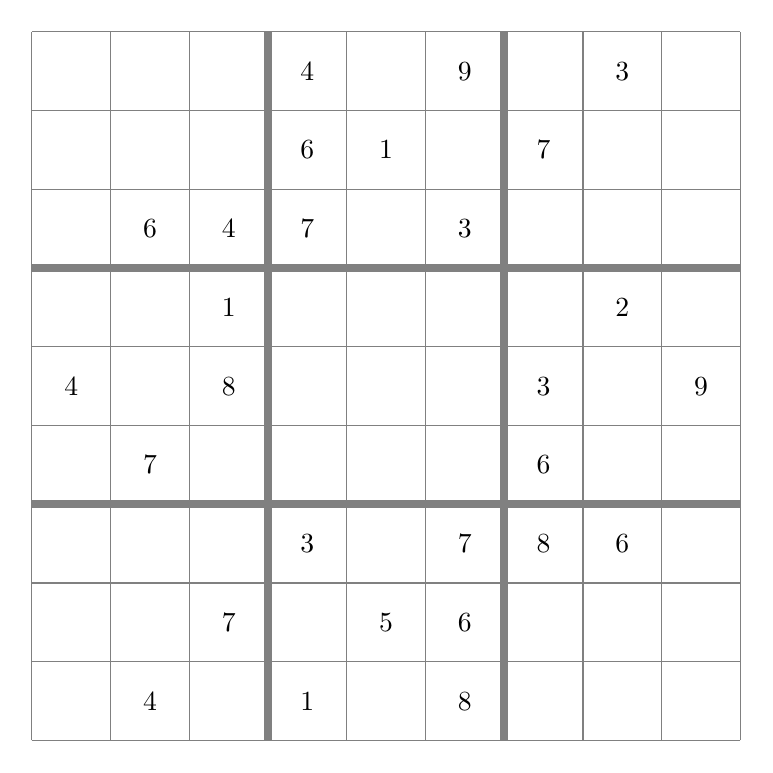
\begin{tikzpicture}
\draw[step=1cm,color=gray] (0,0) grid (9,9);
\draw [line width=3,color=gray] (0,3) -- (9,3);
\draw [line width=3,color=gray] (0,6) -- (9,6);
\draw [line width=3,color=gray] (3,0) -- (3,9);
\draw [line width=3,color=gray] (6,0) -- (6,9);

\node at (1.5,0.5) {4}; \node at (3.5,0.5) {1}; \node at (5.5,0.5) {8};
\node at (2.5,1.5) {7}; \node at (4.5,1.5) {5}; \node at (5.5,1.5) {6};
\node at (3.5,2.5) {3}; \node at (5.5,2.5) {7}; \node at (6.5,2.5) {8}; \node at (7.5,2.5) {6};
\node at (1.5,3.5) {7}; \node at (6.5,3.5) {6};
\node at (0.5,4.5) {4}; \node at (2.5,4.5) {8}; \node at (6.5,4.5) {3}; \node at (8.5,4.5) {9};
\node at (2.5,5.5) {1}; \node at (7.5,5.5) {2};
\node at (1.5,6.5) {6}; \node at (2.5,6.5) {4}; \node at (3.5,6.5) {7}; \node at (5.5,6.5) {3};
\node at (3.5,7.5) {6}; \node at (4.5,7.5) {1}; \node at (6.5,7.5) {7};
\node at (3.5,8.5) {4}; \node at (5.5,8.5) {9}; \node at (7.5,8.5) {3};
\end{tikzpicture}
\end{center}

Your code should write to a file or print to screen its solution and whether the solution is correct.

\noindent Things to consider: 
\begin{itemize}
\item You'll need to generate an initial configuration. 
\item What does a Monte Carlo Step look like for this problem? 
\item What is a good choice of objective function?
\item What values of "temperature" should be used?
\item Make sure the starting numbers are unchanged. 
\end{itemize}

\begin{enumerate}
\item 
\end{enumerate}

\part {2D Ising Model} 


\part{Monte Carlo Atomic }

\noindent Things to Consider: 
\begin{itemize}
\item 
\item 
\end{itemize}

\noindent Optional Extensions: 
\begin{itemize}
\item Compare multiple different cooling schedules. 
\item Have your steps draw from a Gaussian distribution. 
\item 
\end{itemize}

\end{document}  









